% ===========================================================================
% VeriMig -- IEEE conference paper (IEEEtran, 6 pages incl. references)
% Build:  latexmk -pdf main.tex     (or upload the whole paper/ folder to Overleaf)
% Edit text in sections/*.tex, references in refs.bib. See HOW_TO_EDIT.md.
% ===========================================================================
\documentclass[conference]{IEEEtran}
\IEEEoverridecommandlockouts
\usepackage{cite}
\usepackage{amsmath,amssymb}
\usepackage{graphicx}
\usepackage{booktabs}
\usepackage{array}
\usepackage{xcolor}
\usepackage{url}
\usepackage{listings}
\usepackage{algorithm}
\usepackage{algpseudocode}
\usepackage{tikz}
\usetikzlibrary{arrows.meta,positioning}

% ===========================================================================
% defaults.tex -- result macros.
% Every number in the paper is one of these macros. Each defaults to a red [TBD].
% scripts/analyze.py writes tables/macros.tex, which overrides them with real values.
% NEVER type a result number directly into a section file.
% ===========================================================================
\newcommand{\tbd}{\textcolor{red}{\textbf{[TBD]}}}
% corpus
\newcommand{\NumCases}{\tbd}\newcommand{\NumDiffCases}{\tbd}\newcommand{\NumCategories}{\tbd}
\newcommand{\NumSilentCases}{\tbd}\newcommand{\NumControlCases}{\tbd}\newcommand{\NumReviewCases}{\tbd}
\newcommand{\NumPolicyCases}{\tbd}\newcommand{\NumHeldout}{\tbd}
% runs
\newcommand{\NumModels}{\tbd}\newcommand{\NumRuns}{\tbd}\newcommand{\BestModel}{\tbd}
\newcommand{\RulesEquiv}{\tbd}\newcommand{\PlainEquiv}{\tbd}\newcommand{\TrapEquiv}{\tbd}
\newcommand{\AgenticEquiv}{\tbd}\newcommand{\PlainGOne}{\tbd}\newcommand{\AgenticGOne}{\tbd}
\newcommand{\PlainSilent}{\tbd}\newcommand{\AgenticSilent}{\tbd}\newcommand{\PlainSilentGivenCompile}{\tbd}
\newcommand{\PlainSilentClassEquiv}{\tbd}\newcommand{\AgenticSilentClassEquiv}{\tbd}
\newcommand{\PlainCompileClassEquiv}{\tbd}\newcommand{\AgenticCompileClassEquiv}{\tbd}
\newcommand{\McNemarDisc}{\tbd}\newcommand{\McNemarP}{\tbd}
\newcommand{\RepAgreement}{\tbd}\newcommand{\RepairShare}{\tbd}
\newcommand{\PlainTrapDisc}{\tbd}\newcommand{\PlainTrapP}{\tbd}\newcommand{\TrapAgentDisc}{\tbd}\newcommand{\TrapAgentP}{\tbd}
\newcommand{\RulesAgentDisc}{\tbd}\newcommand{\RulesAgentP}{\tbd}
\newcommand{\NumSingleCall}{\tbd}
\newcommand{\CheckEffect}{\tbd}\newcommand{\CheckEffectCI}{\tbd}\newcommand{\RepairEffect}{\tbd}\newcommand{\RepairEffectCI}{\tbd}
\newcommand{\HeldoutRulesEquiv}{\tbd}\newcommand{\HeldoutPlainEquiv}{\tbd}\newcommand{\HeldoutTrapEquiv}{\tbd}
\newcommand{\HeldoutAgenticEquiv}{\tbd}\newcommand{\HeldoutAgenticGOne}{\tbd}\newcommand{\HeldoutTrapGOne}{\tbd}
\newcommand{\HeldoutRepairShare}{\tbd}\newcommand{\HeldoutRuns}{\tbd}\newcommand{\NumDevCases}{\tbd}\newcommand{\MedianSrcLines}{\tbd}\newcommand{\GoSplitShare}{\tbd}\newcommand{\BestAgentSilentShare}{\tbd}
% reconciliation
\newcommand{\RecRowcount}{\tbd}\newcommand{\RecAggregate}{\tbd}\newcommand{\RecRowhash}{\tbd}

% Author-to-author notes (blue). Remove every \note{} before submission.
% Tip: uncomment the next line to hide all notes when checking page count.
% \renewcommand{\note}[1]{}
\newcommand{\note}[1]{\textcolor{blue}{\textit{[Note: #1]}}}

% Include a generated table/figure only once analyze.py has produced it.
\newcommand{\maybeinput}[1]{\IfFileExists{#1}{\input{#1}}{}}

\IfFileExists{tables/macros.tex}{% Generated by scripts/analyze.py -- do not edit by hand.
\renewcommand{\NumCases}{52}
\renewcommand{\NumDiffCases}{50}
\renewcommand{\NumCategories}{16}
\renewcommand{\NumSilentCases}{11}
\renewcommand{\NumControlCases}{5}
\renewcommand{\NumReviewCases}{14}
\renewcommand{\NumPolicyCases}{2}
\renewcommand{\NumHeldout}{6}
\renewcommand{\NumSingleCall}{0}
\renewcommand{\NumDevCases}{46}
\renewcommand{\MedianSrcLines}{5}
\renewcommand{\NumModels}{5}
\renewcommand{\NumRuns}{2116}
\renewcommand{\BestModel}{Qwen2.5C-32B-Q8}
\renewcommand{\RulesEquiv}{56.8}
\renewcommand{\PlainEquiv}{53.0}
\renewcommand{\TrapEquiv}{81.1}
\renewcommand{\AgenticEquiv}{87.9}
\renewcommand{\PlainGOne}{93.5}
\renewcommand{\AgenticGOne}{100.0}
\renewcommand{\PlainSilent}{40.2}
\renewcommand{\AgenticSilent}{12.1}
\renewcommand{\PlainSilentGivenCompile}{43.1}
\renewcommand{\PlainSilentClassEquiv}{50.0}
\renewcommand{\AgenticSilentClassEquiv}{100.0}
\renewcommand{\PlainCompileClassEquiv}{51.2}
\renewcommand{\AgenticCompileClassEquiv}{81.0}
\renewcommand{\McNemarDisc}{1/17}
\renewcommand{\RepAgreement}{97.4}
\renewcommand{\PlainTrapDisc}{2/15}
\renewcommand{\PlainTrapP}{p=0.005}
\renewcommand{\TrapAgentDisc}{0/3}
\renewcommand{\TrapAgentP}{p=0.250}
\renewcommand{\RulesAgentDisc}{2/16}
\renewcommand{\RulesAgentP}{p=0.004}
\renewcommand{\RepairShare}{7.2}
\renewcommand{\CheckEffect}{+28.0}
\renewcommand{\CheckEffectCI}{[+12.1, +43.2]}
\renewcommand{\RepairEffect}{+6.8}
\renewcommand{\RepairEffectCI}{[+0.0, +15.9]}
\renewcommand{\HeldoutRulesEquiv}{33.3}
\renewcommand{\HeldoutPlainEquiv}{33.3}
\renewcommand{\HeldoutTrapEquiv}{66.7}
\renewcommand{\HeldoutAgenticEquiv}{66.7}
\renewcommand{\HeldoutAgenticGOne}{100.0}
\renewcommand{\HeldoutTrapGOne}{100.0}
\renewcommand{\HeldoutRepairShare}{0.0}
\renewcommand{\HeldoutRuns}{276}
\renewcommand{\GoSplitShare}{13.2}
\renewcommand{\BestAgentSilentShare}{100.0}
\renewcommand{\McNemarP}{p<0.001}
\renewcommand{\RecRowcount}{25.0}
\renewcommand{\RecAggregate}{87.5}
\renewcommand{\RecRowhash}{100.0}
}{}

\lstset{basicstyle=\ttfamily\scriptsize,columns=fullflexible,keepspaces=true,frame=single,
  framerule=0.3pt,xleftmargin=2pt,xrightmargin=2pt,aboveskip=3pt,belowskip=3pt}

\begin{document}

\title{VeriMig: A Verification-Gated Agentic LLM Framework for Sybase ASE to SQL Server Migration}

\author{
\IEEEauthorblockN{Sharath Chandra Kampili}
\IEEEauthorblockA{Independent Researcher\\
Texas, USA\\
\note{email}}
\and
\IEEEauthorblockN{Prasad Manda}
\IEEEauthorblockA{Independent Researcher\\
USA\\
prasadmanda.tech@gmail.com}
}

\maketitle

\begin{abstract}
Large language models (LLMs) can translate SAP Adaptive Server Enterprise (ASE) Transact-SQL to
Microsoft SQL Server, but a translation that compiles may still behave differently. We present VeriMig,
a framework that checks each translation with four gates: deployment, a lint for remaining ASE
constructs, differential execution against a reviewed reference translation, and data reconciliation.
Only the first two gates give feedback to the model's repair loop, so the references never shape the
translations they score. We contribute a taxonomy of \NumCategories{} categories of dialect differences,
a corpus of \NumDevCases{} development cases and \NumHeldout{} held-out procedures, and an evaluation of
\NumModels{} locally hosted code models. Without an ASE server, expected behaviour comes from reference
translations; \NumReviewCases{} rely on documented, not executed, ASE semantics.
For the strongest local model, agreement with the references rises from \PlainEquiv\% with a plain prompt
to \TrapEquiv\% with a checklist of known dialect differences and \AgenticEquiv\% with the repair loop.
The checklist improves all five local models; the further gain from repair is not significant. Of the
plain-prompt translations, \PlainSilent\% compile and pass the lint yet disagree with the reference, and on
the held-out procedures agreement is \HeldoutPlainEquiv\% with the plain prompt and
\HeldoutAgenticEquiv\% with the repair loop. A hosted reference model reaches
\HostedPlainEquiv\% with the plain prompt and \HostedTrapEquiv\% with the checklist, so these failures are
mainly a property of smaller local models. A fault-injection study shows that only a per-row hash over an
unambiguous row encoding detects every tested data fault. All artifacts are released.
\end{abstract}

\begin{IEEEkeywords}
database migration, SQL dialect translation, large language models, differential testing,
Sybase ASE, SQL Server, verification, agentic AI
\end{IEEEkeywords}

\section{Introduction}\label{sec:intro}

Many organisations still run business-critical applications on SAP ASE, formerly Sybase, and a common
modernisation path is migration to Microsoft SQL Server. Practitioner guidance describes this path as a
sequence of assessment, planning, schema and code conversion, data movement, testing, cut-over, and
tuning~\cite{manda2026}. Vendor tools such as SQL Server Migration Assistant (SSMA)~\cite{ssma} convert
much of the schema and code, but stored procedures, triggers, and embedded SQL still need manual work, and
most of the effort and risk of a migration sits there.

LLMs can help with that work, but their output is hard to trust. ASE and SQL Server both descend from the
same Transact-SQL code base, so most ASE code is close to valid SQL Server code. Some of the remaining
differences cause compile errors: the ASE \texttt{*=} outer join, for example, is rejected by SQL Server.
Others do not. Under ASE's default settings, \texttt{WHERE col = NULL} matches NULL values, while a SQL
Server procedure created with \texttt{ANSI\_NULLS ON} returns no rows for the same predicate. Concatenating
a NULL with a string gives the string in ASE and NULL in SQL Server. Moving a condition on the inner table
of an ASE outer join into the \texttt{WHERE} clause turns it into an inner join. A migration process that
only checks whether translated code compiles will accept all of these.

This paper studies how well locally hosted LLMs translate ASE code to SQL Server and which checks are
needed before their output can be used. We run the models locally because migration source code often
contains business rules that organisations do not send to external services. Since no ASE server was
available, all results measure agreement with reviewed reference translations; Section~\ref{sec:taxonomy}
explains how the references were built and where they depend on documented ASE behaviour. The paper
contributes:
\begin{enumerate}
\item A taxonomy of \NumCategories{} categories of ASE-to-SQL Server differences, each labelled by how an
unconverted construct shows up, and an open corpus of \NumDevCases{} development cases and \NumHeldout{}
held-out procedures with reference translations (Section~\ref{sec:taxonomy}).
\item VeriMig, a translation framework with four verification gates and a repair loop that never sees the
reference outcomes (Section~\ref{sec:framework}).
\item An evaluation of a rule baseline, plain and checklist prompting, and the repair loop across five
model configurations, with an analysis of the failures that pass compilation
(Sections~\ref{sec:setup}--\ref{sec:results}).
\item A fault-injection study of the data-reconciliation checks used at cut-over, including the encoding
needed for row hashes to be reliable.
\end{enumerate}
We see the benchmark and the failure analysis as the main contributions. The framework combines known
techniques; its value is in how they are arranged and measured for this migration.

\section{Background and Related Work}\label{sec:related}

\textit{Migration practice and tooling.} Manda~\cite{manda2026} surveys the drivers, a staged methodology,
and the risk landscape of ASE-to-SQL Server projects, and recommends record-count and integrity checks
during data validation. That work is descriptive and does not measure conversion correctness or evaluate
automated tooling; VeriMig operationalises its conversion, testing, and validation stages as measurable
gates. Commercial converters---SSMA~\cite{ssma} and the AWS Schema Conversion Tool~\cite{awssct}---translate
schema and much procedural code and report what they cannot convert, while compatibility layers such as
Babelfish~\cite{babelfish} avoid translation by emulating T-SQL on another engine. Rule-based transpilers
such as SQLGlot~\cite{sqlglot} target query dialects rather than ASE procedural semantics.

\textit{LLM-based dialect and code translation.} CrackSQL~\cite{zhou2025cracksql} combines rules with LLM
translation for SQL dialects and reports that pure LLM translation hallucinates functions and fails on long
queries. For general-purpose languages, TransCoder~\cite{roziere2020} evaluated translation by unit tests
rather than token overlap, a point reinforced by the weak correlation between surface metrics such as
CodeBLEU~\cite{ren2020codebleu} and functional correctness. Pan et~al.~\cite{pan2024lost} catalogue the bug
classes LLMs introduce when translating code, many of which compile cleanly. Code-specialised open models
\cite{roziere2023codellama,guo2024deepseekcoder,hui2024qwen} now run on workstations once quantized
\cite{frantar2023gptq,llamacpp}, which makes on-premises translation feasible.

\textit{Self-repair.} Execution and critique feedback improves generated code
\cite{chen2024selfdebug,shinn2023reflexion,madaan2023selfrefine}. We adopt self-repair but deliberately
restrict its feedback channel to signals available without an oracle (Section~\ref{sec:framework}).

\textit{Testing and equivalence.} Differential testing~\cite{mckeeman1998} and its database variants, such
as pivoted query synthesis and query partitioning~\cite{rigger2020pqs,rigger2020tlp}, expose divergence by
comparing executions. Formal SQL provers such as Cosette~\cite{chu2017cosette} cover declarative fragments
but not procedural Transact-SQL with cursors, messages, and errors, so we use observational equivalence
over executed calls.

\section{Dialect-Trap Taxonomy and Corpus}\label{sec:taxonomy}

\textit{Taxonomy.} We derived the taxonomy from the ASE and SQL Server language
references~\cite{aseref,mstsql} and from the authors' migration experience. Each category is labelled by
\emph{observability}: how an unconverted or naively converted construct manifests on SQL Server.
\emph{Compile-visible} traps (C) fail at deployment; \emph{silent} traps (S) deploy and run but change
behaviour; \emph{deprecation} traps (D) behave identically but use features scheduled for removal; and
\emph{control} cases (K) contain already-portable code and measure harmful over-editing.
Table~\ref{tab:taxonomy} summarises the categories and corpus.

\maybeinput{tables/corpus.tex}

\textit{Corpus.} Each case contains (i) the ASE source object a converter sees, (ii) a SQL Server setup
script with target-side tables and data, (iii) a reviewed reference translation, and (iv) one or more calls
whose outcomes define behaviour, chosen to exercise boundary inputs such as NULL arguments, empty strings,
missing keys, and month-end dates. The development corpus holds \NumDevCases{} cases, of which \NumSilentCases{} are silent and
\NumControlCases{} are controls; each isolates one trap and is short. A further \NumHeldout{}
\emph{held-out} composite procedures (7--22 lines, two to five trap categories each, such as a funds transfer or a
batched purge) were written after the trap checklist was frozen and are reported separately. All cases are
synthetic and written by the authors. Two cases encode a migration-policy decision rather than a single
correct behaviour (the result shape that replaces \texttt{COMPUTE BY}, and whether to preserve ASE's
empty-string-as-blank rule); these \NumPolicyCases{} are scored on G1/G2 only, and every other case is scored
differentially on at least two inputs.

Fig.~\ref{fig:trap} shows a silent trap. The ASE procedure keeps customers without large orders; a
translation that moves \texttt{o.amt > 30} into \texttt{WHERE} compiles, passes lint, and drops them.

\begin{figure}[t]
\begin{lstlisting}
-- ASE source
select c.id, c.name, o.amt from cust c, ord o
where c.id *= o.cust_id and o.amt > 30
-- Plausible but wrong (inner-join semantics)
SELECT c.id, c.name, o.amt FROM cust c
LEFT JOIN ord o ON c.id = o.cust_id WHERE o.amt > 30
-- Reference: restriction stays in the join
SELECT c.id, c.name, o.amt FROM cust c
LEFT JOIN ord o ON c.id = o.cust_id AND o.amt > 30
\end{lstlisting}
\caption{A silent outer-join trap (corpus case C02).}
\label{fig:trap}
\end{figure}

\textit{Reference validation.} Every reference translation must deploy on SQL Server 2022 and produce its
expected outcomes before any run starts; a failing reference aborts the experiment. For the
\NumReviewCases{} cases whose expected behaviour depends on ASE-specific semantics, that behaviour is
derived from the ASE 16 documentation~\cite{aseref} under default server options, and the cases are flagged
in the artifact for re-checking against a live instance \note{if you execute them on ASE, say so here with
the version, e.g. ``and confirmed by executing the sources on ASE 16.0 SP04''}.

\section{The VeriMig Framework}\label{sec:framework}

Fig.~\ref{fig:arch} shows the pipeline. Each ASE object is paired with the checklist of known
differences, translated by a converter, and checked by four gates. We study four converters: a
deterministic rule baseline, an LLM with a plain prompt, an LLM with the checklist added to the prompt, and
the same LLM with a repair loop.

\begin{figure}[t]
\centering
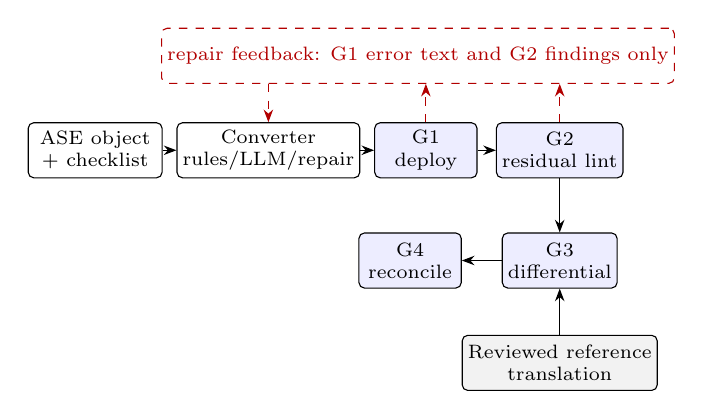
\begin{tikzpicture}[font=\scriptsize, x=1mm, y=1mm,
  box/.style={draw, rounded corners=2pt, align=center, minimum height=7mm, inner sep=2pt},
  gate/.style={box, fill=blue!7, minimum width=13mm},
  arr/.style={-{Stealth[length=1.6mm]}}]
\node[box, minimum width=17mm] (src) at (0,0) {ASE object\\+ checklist};
\node[box, minimum width=19mm] (conv) at (22,0) {Converter\\rules/LLM/repair};
\node[gate] (g1) at (42,0) {G1\\deploy};
\node[gate] (g2) at (59,0) {G2\\residual lint};
\node[gate] (g3) at (59,-14) {G3\\differential};
\node[gate] (g4) at (40,-14) {G4\\reconcile};
\node[box, fill=gray!10, minimum width=22mm] (ref) at (59,-27) {Reviewed reference\\translation};
\node[box, dashed, draw=red!70!black, text=red!70!black, minimum width=50mm] (fb) at (41,12)
  {repair feedback: G1 error text and G2 findings only};
\draw[arr] (src) -- (conv);
\draw[arr] (conv) -- (g1);
\draw[arr] (g1) -- (g2);
\draw[arr] (g2) -- (g3);
\draw[arr] (g3) -- (g4);
\draw[arr] (ref) -- (g3);
\draw[arr, dashed, red!70!black] (g1.north) -- (g1.north |- fb.south);
\draw[arr, dashed, red!70!black] (g2.north) -- (g2.north |- fb.south);
\draw[arr, dashed, red!70!black] (conv.north |- fb.south) -- (conv.north);
\end{tikzpicture}
\caption{VeriMig pipeline. Dashed arrows show the only feedback the repair loop receives; the reference
used by G3 never reaches the converter.}
\label{fig:arch}
\end{figure}

\textbf{G1 (deploy).} The candidate is executed batch by batch in a new SQL Server database after the case
setup. Session options are fixed (\texttt{ANSI\_NULLS}, \texttt{QUOTED\_IDENTIFIER}, and
\texttt{CONCAT\_NULL\_YIELDS\_NULL} on), matching current client defaults.

\textbf{G2 (residual lint).} Eighteen pattern rules detect ASE constructs that should not remain after
translation, such as \texttt{*=}, \texttt{@@sqlstatus}, \texttt{\%1!} placeholders, unbracketed lock hints,
unsigned and \texttt{big*} types, and lock-scheme clauses. Error-level findings fail the gate; deprecated
but valid types are recorded as warnings. Some silent categories, such as the GROUP BY extension and NULL
concatenation, cannot be detected by patterns.

\textbf{G3 (differential).} The reference and the candidate are deployed in separate databases with the
same setup, and every call runs in both. The candidate passes if, for every call, the following match:
all result sets in order (rows are compared as multisets only when a case declares that order does not
matter), with exact values and no rounding; the procedure's return code, captured by wrapping each
single-procedure call; whether an error was raised and its message text; informational messages, where the
case declares them; and the transaction state after the call (\texttt{@@TRANCOUNT} and
\texttt{XACT\_STATE()}). After the last call, the final contents of every user table must also match, so
side effects that no call selects are still checked; \texttt{rowversion} columns are excluded because their
values are database counters. Column names and error numbers are not compared, since a correct translation
may rename an output column or use a different user error number. Every procedure with output parameters
has calls that read them back, which an automated test enforces. Interface metadata, meaning each
procedure's parameter names, types, and output flags and the column types of each result set, is compared
with the reference and reported separately, because a correct translation may legitimately widen a type
(for example, \texttt{unsigned int} to \texttt{bigint}). The comparison shows agreement on the chosen inputs; it is not a proof of
equivalence.

\textbf{G4 (reconcile).} During data movement, VeriMig compares source and target tables. We evaluate four
detectors: row counts; SQL Server's aggregate checksum, \texttt{CHECKSUM\_AGG(BINARY\_CHECKSUM(*))}, which
combines a 32-bit checksum per row into one value by an algorithm Microsoft does not document in detail;
and two per-row SHA-256 hashes. The naive hash joins column values with a separator and writes NULL as a
marker string, which is ambiguous: NULL and the text \texttt{<NULL>} produce the same input, as do
(\texttt{A|B}, \texttt{C}) and (\texttt{A}, \texttt{B|C}). The unambiguous hash writes each column as
\texttt{N;} for NULL or \texttt{V}\emph{length}\texttt{:}\emph{value}\texttt{;} otherwise, converts values
with \texttt{nvarchar(max)} so nothing is truncated, and uses explicit conversion styles for date, time,
and money columns. Distinct rows therefore always produce distinct hash inputs. Rows are compared as a
multiset of (key, hash) pairs, so missing and duplicate keys are also found.

\textbf{Oracle-separated repair.} Algorithm~\ref{alg:agent} gives the repair loop. It receives only the SQL
Server error text from G1 and the remaining ASE constructs from G2, never G3 outcomes. In a real migration
there is no reference for a customer's procedure, and keeping G3 out of the loop prevents the measured
agreement from being tuned against the evaluation signal.

\begin{algorithm}[t]
\caption{Oracle-separated repair loop}\label{alg:agent}
\footnotesize
\begin{algorithmic}[1]
\Require ASE object $s$, model $M$, checklist $T$, budget $K$
\State $h \gets [\textsc{System}(T), \textsc{User}(s)]$
\For{$i = 1$ \textbf{to} $K$}
  \State $c \gets \textsc{Extract}(M(h))$
  \State $(ok_1, e) \gets \textsc{G1}(c)$;\ \ $(ok_2, f) \gets \textsc{G2}(c)$
  \If{$ok_1 \wedge ok_2$} \textbf{break} \EndIf
  \State $h \gets h \Vert [c, \textsc{Feedback}(e, f)]$ \Comment{no G3 signal}
\EndFor
\State \Return $c$ \Comment{then scored once by G1--G3}
\end{algorithmic}
\end{algorithm}

\section{Experimental Setup}\label{sec:setup}

\textit{Research questions.}
\textbf{RQ1:} How often do translations from each converter deploy, pass the lint, and agree with the
reference?
\textbf{RQ2:} What share of translations passes G1 and G2 but fails G3?
\textbf{RQ3:} Which categories remain hard, and where do the remaining failures come from?
\textbf{RQ4:} How do model size and quantization affect agreement and latency on local hardware?
\textbf{RQ5:} Which reconciliation checks detect injected data faults?

\textit{Platform.} All experiments ran on one Mac Studio (\HwChip) with \HwMemory{} of unified memory
(\HwCores{} cores) under macOS \HwMacOS. SQL Server 2022 Developer Edition (build \SqlBuild) ran in Docker
\DockerVersion{} as the \texttt{amd64} image \texttt{mcr.microsoft.com/mssql/server} (digest \texttt{\ImageDigest}) under
Rosetta emulation. Models were served by Ollama~\cite{ollama}, which
uses llama.cpp~\cite{llamacpp}. We evaluate \NumModels{} configurations from two model
families~\cite{hui2024qwen,deepseek2024v2}: Qwen2.5-Coder at 7B, 14B, and 32B with 4-bit quantization
(Q4\_K\_M), the 32B model with 8-bit quantization (Q8\_0), and DeepSeek-Coder-V2 Lite, a 16B
mixture-of-experts model with 4-bit quantization (Q4\_0). Model digests are recorded in the artifact.
\maybeinput{tables/hosted_setup.tex}

\textit{Converters.} The rule baseline applies 22 regular-expression rewrites and normalises quotes; it
covers the lint-visible categories and deliberately does not restructure joins or grouping, so it is a
lower bound rather than a substitute for a commercial converter. The plain prompt asks for a translation
that preserves behaviour. The checklist prompt adds one line per G2 rule and three lines for silent
categories that the lint cannot detect. The repair loop runs Algorithm~\ref{alg:agent} with $K=3$.
Temperature is 0.2 with fixed seeds, and each LLM configuration runs three times per case; the rule baseline
is deterministic and runs once. The held-out set therefore has 276 graded runs: 6 procedures, each
translated by 5 models with 3 LLM converters 3 times (270), plus 6 rule-baseline runs.

\textit{Prompts.} Both prompts share the instruction below (shortened); the full text is in the artifact.
\begin{lstlisting}
You are an expert database migration engineer.
Translate SAP ASE (Sybase) Transact-SQL into
Microsoft SQL Server 2022 Transact-SQL. Preserve
the runtime behaviour of the original exactly
(same result sets, same NULL handling, same
errors raised). Keep object names unchanged.
Return only the translated code in a single
sql block.
\end{lstlisting}

\textit{Metrics.} G1 and G2 rates are computed over all cases and G3 agreement over cases scored
differentially. The \emph{silent} rate is the share of differential runs that pass G1 and G2 but fail G3.
The three seeds gave the same G3 outcome in \RepAgreement\% of case and configuration pairs, so we treat the
case, not the run, as the unit of analysis: intervals are 95\% bootstrap confidence intervals (CIs) over
cases (10{,}000 resamples)~\cite{efron1993}, and paired comparisons use the exact McNemar
test~\cite{mcnemar1947} on per-case majority outcomes. Latency is the wall-clock time of the model calls
for one case; for the repair loop it also includes the G1 and G2 checks between attempts, but never G3.

\textit{Model selection.} The ``strongest model'' is chosen from the results, as the configuration with the
highest agreement for the repair loop. Statistical tests on that model are therefore exploratory. To show
that the main result does not depend on this choice, we also test the checklist effect for every model,
with Holm correction across models.

\textit{Test adequacy.} To measure how well the inputs detect behaviour changes, we applied 23 mutation
operators to the reference translations, each making one small change of the kind seen in failed
translations (for example \texttt{IS NULL} to \texttt{= NULL}, a left join to an inner join, removing an
\texttt{ISNULL}, widening a comparison, narrowing a type, changing an error message, or dropping a
\texttt{COMMIT}). This gives \MutTotal{} mutants. A mutant is detected if it fails G1 or G3 against the
unchanged reference; we inspected every mutant that was not detected.

\textit{G4 protocol.} A seeded 2{,}000-row table with Unicode names, names containing the separator
character, 4-decimal money values, microsecond timestamps, and nullable text values of up to 6{,}000
characters is loaded as the source. For each fault type and each of \RecTrials{} trials, the target
receives one injected fault. Most faults change one row; swapping amounts between two rows changes two.
Four faults are aimed at the naive encoding: a NULL replaced by the text \texttt{<NULL>}, a value moved
across the separator between two columns, a change at the end of a value longer than 4{,}000 characters,
and one row's key replaced by another row's key. Clean trials measure false positives. Source and target
are both on SQL Server, so the study measures detector sensitivity, not cross-engine extraction.

\section{Results}\label{sec:results}

\maybeinput{tables/main_results.tex}

\textit{RQ1: gate pass rates.} Table~\ref{tab:main} reports every configuration. For the strongest model
(\BestModel), behavioural equivalence rises from \PlainEquiv\% with the plain prompt to \TrapEquiv\% with the
trap-aware prompt and \AgenticEquiv\% with the agent, against \RulesEquiv\% for the rule baseline; deployment
success rises from \PlainGOne\% to \AgenticGOne\%. The checklist is the significant ingredient: it adds \CheckEffect{} points of
case-level equivalence (95\% CI \CheckEffectCI; plain-only/trap-only correct \PlainTrapDisc, Holm-adjusted
$\PlainTrapP$), whereas repair adds \RepairEffect{} (\RepairEffectCI; $\TrapAgentP$). The repair loop ran in
\RepairShare\% of agentic runs; on these short cases it is a small, non-significant addition. The agent still
beats the rule baseline ($\RulesAgentP$). Size does not help without the checklist: with the plain prompt the
14B model outperforms both 32B variants. The 32B models translate near-literally, carrying ASE semantics
across whenever the code still compiles, and in a few runs split a procedure with \texttt{GO}
(\GoSplitShare\% of plain-prompt deployment failures)---plausibly prompted by the instruction to separate
batches with \texttt{GO}. With the checklist, the 32B models lead, though their intervals overlap the 14B
model's.

\textit{RQ2: the silent share.} Of plain-prompt translations from the strongest model that deployed,
\PlainSilentGivenCompile\% were behaviourally wrong. Overall, \PlainSilent\% of its plain runs and
\AgenticSilent\% of its agentic runs passed G1 and G2 yet failed G3. For the agent, \BestAgentSilentShare\%
of all remaining failures are silent: the gates removed every failure they can observe, and what is left is
exactly the class that only differential testing exposes.

\maybeinput{tables/observability.tex}

\textit{RQ3: what stays hard.} Table~\ref{tab:observability} splits equivalence by trap class, with a
counter-intuitive result. The agent scores \AgenticSilentClassEquiv\% on traps \emph{labelled} silent
(plain: \PlainSilentClassEquiv\%), because the checklist names them, but \AgenticCompileClassEquiv\% on
compile-visible traps (plain: \PlainCompileClassEquiv\%), where the \emph{repair} of a construct that will
not compile often produces code that compiles but behaves differently:
the GROUP BY extension is ``fixed'' by grouping or partitioning per row (C10, C28), a legacy right outer
join is rewritten with the wrong preserved table (C29), and unsigned types are narrowed to same-width
signed types that overflow on real values (C35, C36). In other words, fixing a loud error is a common
source of a quiet one.

\maybeinput{tables/failures.tex}

\textit{Error analysis.} Table~\ref{tab:failures} lists the cases that most often slipped past G1 and G2.
Two further patterns recur across models. First, surface rewriting can defeat lint while keeping the bug:
one model translated \texttt{mgr\_id = null} as \texttt{mgr\_id = convert(int, null)}, which passes the
\texttt{= NULL} rule and still returns no rows (C08). Second, error translation is fragile:
\texttt{raiserror (20001, 16, 1, ...)} raises SQL Server's built-in replication message 20001 rather than
the intended text, and \texttt{THROW} rejects ASE's user-error range outright (C05).

\IfFileExists{figures/category_g3.pdf}{%
\begin{figure}[t]\centering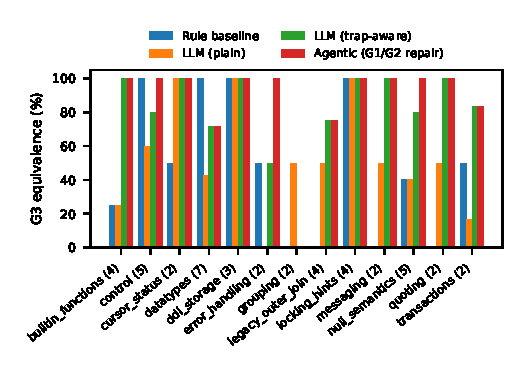
\includegraphics[width=\columnwidth]{figures/category_g3.pdf}
\caption{G3 equivalence by trap category for the strongest model.}\label{fig:cat}\end{figure}}{}

\textit{Held-out procedures.} On the \NumHeldout{} composite procedures (\HeldoutRuns{} graded runs), the
strongest model reaches \HeldoutPlainEquiv\% with the plain prompt, \HeldoutTrapEquiv\% with the checklist,
and \HeldoutAgenticEquiv\% with the agent (rule baseline: \HeldoutRulesEquiv\%). Deployment success is
\HeldoutTrapGOne\% for the trap-aware prompt and \HeldoutAgenticGOne\% for the agent, which repaired
\HeldoutRepairShare\% of these longer translations.
\note{After the held-out runs: one sentence on whether the checklist still helps on code it was not written
from, and whether repair matters more here than on single-trap cases.}

\textit{RQ4: size, quantization, and cost.} Fig.~\ref{fig:scaling} plots equivalence against mean latency
per case. The 4-bit and 8-bit 32B models reach the same agentic equivalence, while the 8-bit model is
slower, so on this hardware 4-bit quantization costs no measured accuracy. The 14B model trails slightly at lower latency,
and the second model family is weakest under every converter. Every configuration translates a case in seconds on a single
workstation.

\IfFileExists{figures/scaling.pdf}{%
\begin{figure}[t]\centering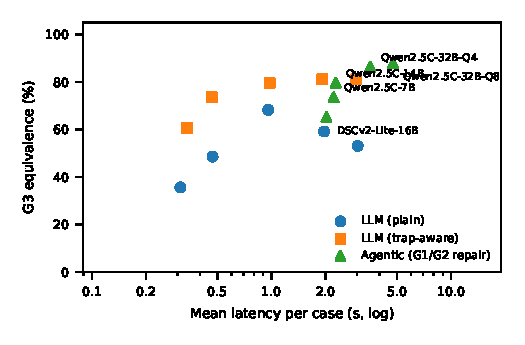
\includegraphics[width=\columnwidth]{figures/scaling.pdf}
\caption{Equivalence versus mean latency per case; labels mark agentic runs per model.}\label{fig:scaling}\end{figure}}{}

\maybeinput{tables/reconcile.tex}

\textit{RQ5: reconciliation.} Across injected single-row faults, row counts detect \RecRowcount\%, the
aggregate checksum \RecAggregate\%, and per-row hashing \RecRowhash\%, with no false positives on clean
trials (Table~\ref{tab:reconcile}). Row counts see only faults that change cardinality, so the content
faults typical of type-mapping errors---truncation, charset loss, rounding, precision loss---all pass a
count-only check. The aggregate checksum catches those but misses every swap of values between rows, which is
consistent with an order-insensitive, XOR-like combination of row checksums (the algorithm is not
documented). Only per-row hashing detects every fault.

\section{Discussion and Threats to Validity}\label{sec:discussion}

\textit{Implications for practice.} Compile success is a weak acceptance criterion for LLM-translated
database code, and so is lint: once the obvious constructs are gone, the remaining defects are precisely
the ones neither check can see, and a model may even rewrite a flagged construct into an equivalent
unflagged one. Three practices follow from our results. First, give the model the dialect knowledge
explicitly; a trap checklist was worth more than a larger model or a repair loop. Second, treat every \emph{repair} of a
compile error as suspect, since that is where the agent's residual silent errors arose; such objects
deserve differential tests or human review before cut-over. Third, reconcile migrated data with per-row
hashes rather than counts or aggregate checksums. All three run on a single workstation with local models,
so source code never leaves the organisation.

\textit{Oracle errors.} We manually audited every silent failure. The audit found one reference
translation (C06) that contradicted ASE's NULL-concatenation rule and no others; we corrected it and
re-scored the stored translations without regenerating them. \textit{Corpus.} All cases are synthetic and written by the authors, who also wrote the trap checklist;
development results for trap-aware prompting are therefore an upper bound. The held-out procedures,
written after the checklist was frozen, estimate how it generalises, but six procedures are a small sample.
\textit{Test adequacy.} Every differentially scored case runs on two to four inputs chosen to exercise NULLs,
empty tables and edge values; a candidate can still match on these and diverge elsewhere, so G3 results
remain optimistic.
\textit{Baselines.} The rule baseline was written by the authors and is a lower bound; SSMA was not
evaluated. \textit{Oracle.} References encode one acceptable target behaviour; a correct but differently shaped
translation (e.g., reordered result sets) can fail G3, while renamed output columns are tolerated.
\textit{Engine versions.} ASE semantics vary with version and server options (e.g., \texttt{ansinull},
chained mode); we assume ASE 16 defaults and SQL Server 2022 with modern client defaults.
\textit{Isolation semantics.} Single-session differential testing cannot observe concurrency effects such
as a lock hint mapped to \texttt{NOLOCK}; such candidates need review.
\textit{Model nondeterminism.} Seeds barely changed outcomes (\RepAgreement\% agreement), so we report case-level intervals rather than treating repetitions as independent.
\textit{Reconciliation.} G4 runs with both tables on SQL Server; it measures detector sensitivity, not
end-to-end transfer tooling.

\section{Conclusion}\label{sec:conclusion}

LLMs can translate much of an ASE code base to SQL Server, but a translation that compiles is often wrong
in ways that only execution shows. In our study, an explicit checklist of dialect differences improved
every local model, a repair loop added little, and nearly all remaining errors passed compilation and lint.
A hosted model made almost none of these errors, which shows both how much depends on model capability
and that harder benchmarks are needed.
VeriMig makes these errors visible by comparing each translation with a reviewed reference on several inputs
and by reconciling migrated data with an unambiguous row hash. Future work will validate the references on a
live ASE server, add SSMA as a baseline, and extend the corpus with independently written production
procedures.

\section*{Artifact Availability}
Code, corpus, prompts, raw run logs, and analysis scripts are available at
\url{https://github.com/sharath568/verimig}. Release \texttt{v1.1-camera-ready} matches the results in
this paper; earlier results were superseded by the corrections described in Section~\ref{sec:discussion}.


\bibliographystyle{IEEEtran}
\bibliography{refs}

\end{document}
